\subsection{Diseño del algoritmo}

En el presente informe se detalla la implementación de una herramienta para procesar señales moduladas en amplitud, de acuerdo al siguiente esquema:

\begin{figure}[h]
\centering
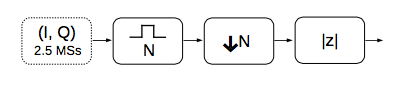
\includegraphics[width = 0.6 \textwidth]{flujo_senales}
\caption{Flujo de procesamiento de señales.}
\label{fig:flujo_senales}
\end{figure}

Se provee como entrada una secuencia de números complejos $(I[n],Q[n])$ que representan las muestras en fase y cuadratura de la señal modulada. Esta secuencia se pasa por un \textit{moving average}, un decimador y finalmente se le calcula el módulo punto a punto para obtener a la salida una secuencia de números reales $R[n']$.

En primer lugar se definió el algoritmo mediante el cual se realizaría el procesamiento de señales. 

Se tuvo en cuenta el hecho de que, a partir del \textit{downsampling}, se desecha una cantidad importante de muestras. Específicamente, si se fijó un parámetro de decimación $N$, de cada $N$ muestras procesadas sólo una es finalmente utilizada. Por lo tanto sólo hace falta realizar los cálculos para las muestras que sabemos van a ``sobrevivir'' la decimación.

Para cada muestra $n$, el \textit{moving average} realiza un promedio de las $N$ últimas muestras recibidas, es decir sigue la ecuación:

	\begin{equation*}
		 y[n] = \frac1N \sum_{k = 0}^{N-1} x[n-k]. 
	\end{equation*}

De lo anterior se sigue que cada muestra a la salida $y[n_0]$ es sólo función de los $N$ últimos valores a la entrada $x[n_0], x[n_0 - 1], \dots,  x[n_0 - N + 1]$. Los demás bloques de procesamiento sólo dependen del valor actual de su entrada, por lo que finalmente en el programa sólo hace falta recordar las últimas $N$ muestras que se recibieron para realizar los cálculos. 

Con estas observaciones en mente, se optó por el siguiente algoritmo de implementación:

	\begin{algorithmic}[H] % algorithmic fue el que pude hacer andar, porque me dejaba 
		       % redefinir las keywords. algorithm2e era mas lindo pero seteandolo
                       % con spanish y onelanguage mezclaba español con italiano.
		       % Si encontras uno que se vea mejor y en español es bienvenido.

		%\caption{Algoritmo para el procesamiento de las muestras.}
	
		\While{el \textit{stream} de datos no termine}
			\State $promedio := 0$
			\For{las N siguientes muestras}
				\State $promedio \gets promedio + x[n]$
			\EndFor
			\State $promedio \gets promedio / N$
			\Return $\sqrt{\mathbf{Re}\{promedio\}^2 + \mathbf{Im}\{promedio\}^2}$ 
		\EndWhile
	\end{algorithmic}

\newpage

\subsection{Implementación}
 De acuerdo a lo requerido, la implementación de la herramienta se realizó en C++, para entradas y salidas de texto en los formatos especificados. Para ello se aprovecharon las clases \texttt{cmdline} y \texttt{complex} provistas en el curso, para el manejo de argumentos y números complejos respectivamente.

 Con respecto al manejo de argumentos, para utilizar la clase \texttt{cmdline} hace falta definir la tabla de opciones que se esperan recibir, de tipo \texttt{option\_t}. Se optó por definirla dentro del \texttt{main} del programa, con las siguientes opciones:

\lstset{language=C++}
\begin{lstlisting}[frame=single]
static option_t options[] = {
	{1, "i", "input", "-", opt_input, OPT_DEFAULT},
	{1, "o", "output", "-", opt_output, OPT_DEFAULT},
	{1, "N", "n_decimator","500",opt_n_decimator, OPT_DEFAULT},
	{0, "h", "help", NULL, opt_help, OPT_DEFAULT},
	{0, },
\end{lstlisting}

Como es requerido, se definió a la cadena ``-'' (tercera columna de la tabla de opciones) como el valor por defecto para las opciones de entrada y de salida. De esta manera, ya sea que se haya omitido esa opción o se la especifique explicítamente para que asuma su valor por defecto, en ambos casos se  obtendrá el mismo resultado.

Además la clase \texttt{cmdline} pide especificar las funciones que se utilizarán para parsear cada opción (5ta columna de la tabla) - se las definió en el mismo \texttt{main}. Para las funciones que parsean las opciones de entrada, salida y ayuda se aprovecharon las que ya estaban implementadas en el archivo \texttt{main.cc} provisto con la implementación de la clase \texttt{cmdline} del curso. Quedó por definir, entonces, el \texttt{parser} para el parámetro $N$ de decimación:


\lstset{language=C++} % Esta seteado para utf8 pero no puede renderear los acentos! No entiendo por que
\begin{lstlisting}[frame=single]
static void
opt_n_decimator(string const &arg)
{
	istringstream iss(arg);

	// Intentamos extraer el N de la linea de comandos.
	// Para detectar argumentos que unicamente consistan de
	// numeros enteros, vamos a verificar que EOF llegue justo
	// despues de la lectura exitosa del escalar
	
	if(!(iss >> n_decimator) || !iss.eof()) {
		cerr << "non-integer factor: "
		     << arg
		     << "."
		     << endl;
		exit(1);
	}

	if (iss.bad()) {
		cerr << "cannot read integer factor."
		     << endl;
		exit(1);
	}
}
\end{lstlisting}

Como el método \texttt{parse} de \texttt{cmdline} ya le pasa al \texttt{parser} su valor por defecto si fue omitido, siempre esta función recibirá un argumento para $N$ (no necesariamente válido). Se intenta leer el mismo como un entero, y de fallar se anuncia el error y se termina el programa. 

Los argumentos se leen mediante \texttt{cmdline.parse($\cdot$)} a cada una de las variables estáticas definidas fuera del \texttt{main}:

 
\lstset{language=C++}
\begin{lstlisting}[frame=single]
static size_t n_decimator;	// Decimator Factor (factor positivo de decimacion)
static istream *iss = 0;	// Input Stream (clase para manejo de los flujos de entrada)
static ostream *oss = 0;	// Output Stream (clase para manejo de los flujos de salida)
static fstream ifs; 		// Input File Stream (derivada de la clase ifstream que deriva de istream para el manejo de archivos)
static fstream ofs;		// Output File Stream (derivada de la clase ofstream que deriva de ostream para el manejo de archivos)
\end{lstlisting}

Estas son las variables que se le pasan a \texttt{am\_proc} que es la encargada de implementar el algoritmo de la sección anterior, de manera que el \texttt{main} queda:


\lstset{language=C++}
\begin{lstlisting}[frame=single]
int
main(int argc, char * const argv[])
{
	cmdline cmdl(options);	// Objeto con parametro tipo option_t (struct) declarado globalmente.
	cmdl.parse(argc, argv);	// Metodo de parseo de la clase cmdline
	am_proc(iss, oss, n_decimator);	// Procesamiento AM
}
\end{lstlisting}

La función \texttt{am\_proc} está declarada en ``\texttt{am\_proc.h}'' y definida en ``\texttt{am\_proc.cc}''. Fuera de chequear por errores de lectura, su implementación es en escencia el pseudo-código de la sección anterior:

\lstset{language=C++}
\begin{lstlisting}[frame=single]
void am_proc(istream *is, ostream *os, const size_t& n_decimator){
	
	bool eof_flag=false;
	size_t i;
	complejo c, aux; // c tendra la suma y aux sera el que recibe el complejo del stream	


	// Si entra un archivo vacio (primero lee EOF), corta el for y luego el while, devolviendo un vacio

	while(!eof_flag){
		
		// Se suman los primeros 'n_decimator' numeros hasta que corte 
		for(i=1; i<=n_decimator && ((*is)>>aux); i++)
			c += aux;
	
		// Compruebo si se llego a EOF
		if(is->eof())
			eof_flag=true;

		if(is->bad()){ 
		// El for termino por no poder guardar el caracter en x
			cerr	<< "Error: Cannot read complex on input stream"
				<< endl;
			exit(1);
		}		

		// Realizo el proemdio movil
		c=c / n_decimator;
			
		// Imprimo el valor absoluto
		*os << c.abs()<<endl;
	}
	
	if(os->bad()){
		cerr	<< "Error: Cannot write output file"
			<< endl;
		exit(1);
	}

}
\end{lstlisting}

